\documentclass[12pt]{article}
\usepackage{fullpage,graphicx,psfrag,amsmath,amsfonts,verbatim}
\usepackage[small,bf]{caption}
\usepackage{amsthm}
\usepackage[hidelinks]{hyperref}
\usepackage{bbm} % for the indicator function to look good
\usepackage{color}
\usepackage{mathtools}
\usepackage{fancyhdr} % for the header
\usepackage{booktabs} % for regression table display (toprule, midrule, bottomrule)
\usepackage{adjustbox} % for regression table display
\usepackage{threeparttable} % to use table notes
\usepackage{natbib} % for bibliography
\input newcommand.tex
\bibliographystyle{apalike}
% \setlength{\parindent}{0pt} % remove the automatic indentation

\title{L'Hopital's (Selection) Rule:\\{\large {An Empirical Bayes Application to French Hospital Efficiency}}}
\author{Fu Zixuan \\{\small {Supervised by Thierry Magnac}}}
\date{July 4, 2024}

\begin{document}
\maketitle
\thispagestyle{empty}
\begin{abstract}
    \noindent  Something interesting\\

    % \noindent\textbf{Keywords:} \\

    \bigskip
\end{abstract}

\newpage
\thispagestyle{empty}
\tableofcontents
\newpage

\setcounter{page}{1}
\section{Introduction}

It is almost of human nature to compare, rank and select. And competition, be
it good or bad, emerges in the wake. As invidious as ranking and selection can
be, in many cases it is one of the driving forces behind improvement in
performances. The society itself is constantly constructing league table as
well. It rewards the meritorious and question or even punishes the
unsatisfactory. The measure based on which rank is constructed ranges from
teacher's evaluation \citep{chetty2014measuring}, communities' mobility index
\citep{chetty2018impacts} to firm discrimination \citep{kline2022systemic}.

The present article extends the practice to the health sectors. To be more
specific, it studies the labor efficiency across all hospitals in France. By
exploring a comprehensive database called \textit{The Annual Statistics of
    Health Establishments (SAE)} of French hospitals, I first construct a measure
of labor efficiency. Then based on the estimates, we compare the public and
private hospitals by selecting the top-performing units. I borrow from the
recent developments in Empirical Bayes method to achieve the comparison.

I found that out of the top 20\% best performing hospitals, there are roughly 5
times more private units than the public, adjusted by the number of hospitals
in each category. The difference is more pronounced when I also control for the
expected number of wrongly selected. The takeaway is that public hospitals are
in general less efficient than private ones. While the conclusion is in line
with that of \cite{croiset2024hospitals} that, now we have a granular
perspective on the performance comparison.

The article bridges two fields of interests. The first one is on productivity
analysis. The most popular methods in the field are Data Envelopment Analysis
\citep{charnes1978measuring} and Stochastic Frontier Analysis
\citep{aigner1977formulation,meeusen1977efficiency}. Yet I abstract from both
of them and use the \textit{conditional input demand function} specification
stated in \cite{croiset2024hospitals}.\footnote{I refer the reader to
    \citet{croiset2024hospitals} for detailed reasons of adopting such an
    approach.} To put it simply, we estimate a linear function of how much labor
input is needed to produce a give list of 8 hospital outputs. I only focus on
the employment level of nurses because unlike medical doctors, this is a
category that do not suffer from a shortage of labor supply.

The second area of interests is the Empirical Bayes Methods. I lean on a series
of work by Jiaying Gu and Roger Koenker, chiefly the following two papers.
\citet{gu2017empirical} discussed the usefulness of estimating a prior
distribution in baseball batting average prediction. And
\citet{gu2023invidious} has formally defined the selection problem as a
compound decision on which the estimated prior can be of help as well.
\citet{kiefer1956consistency} has shown that non parametric maximun likelihood
estimation of the prior is feasible and consistent. The computation of NPMLE is
greatly improved by \citet{koenker2014convex} by leveraging the recent
development in convex optimization \citep{andersen2010mosek}. I will be using
the \verb+REBayes+ package \citep{koenker2017rebayes} in the estimation, which
is based on software \verb+MOSEK+ developed by \citet{andersen2010mosek}.

In \cite{croiset2024hospitals}, the authors argue that public hospital is less
efficient than private counterpart in the sense that it would need a smaller
size of personnel if it were to use the input demand function of the private
hospital, which is the main result of their counterfactuals.

Having roughly replicated the results after doubling the length of the panel,
the paper differentiates itself by utilizing classical panel data methods in
input demand function estimation, specifically the standard fixed-effect
estimation and GMM. Though it is straightforward to include individual fixed
effect in specification, estimation is not without challenge. For example, as
\citet{croiset2024hospitals} has correctly pointed out, within hospital
variation is much smaller than between group variation. The former may be
insufficient to obtain credible estimates. I extended the panel length in an
attempt to mitigate the problem. Secondly, the strict exogeneity assumption
required by the standard within group estimation is questionable. A natural way
to relax it is to use the first difference GMM estimator proposed by
\citet{arellano1991some}. The high persistency in the regressors poses another
challenge of weak instruments. In response,
\citet{arellano1995another,blundell1998initial}'s system GMM is modified and
implemented, and the estimation results are used for the rest of the section.

The benefit of the panel data estimator is that it gives us an estimate of the
underlying heterogeneity, which opens door to individual comparisons. However,
the fixed effect estimates are generally noisy, rendering the ensuing decision
maker hand wavy in making choices. The EB methods are proposed in an attempt to
rectify the situation by empirically estimating the prior distribution of the
fixed effect.

For example, in \cite{gu2023invidious}, we are given the task of selecting the
top 20\% fixed effect denoted by $\theta_i$. If the $\theta_i$ follows a
distribution $G$, this is to say we are selecting those $\theta_i>G^{-1}(0.8)$.
The decision rule for individual $i$ is an indicator function $\delta_i$,
determining whether $i$ belongs to selection set. The task naturally falls
under the compound decision framework pioneered by \cite{herbert1956empirical}
if we define the loss function of the selection problem in such a way that
takes into account the results of all the individual decisions $\delta_i$.
\begin{equation*}
    \delta^* = \argmin_{\delta} \E_G\E_{\theta|\hat{\theta}}\pa{L_n}.
\end{equation*}
Since we don't know the true value $\theta$, we minimize the expected compound loss  $L_n$ over the distribution of $\theta$ given the observed $\hat{\theta}$.

In addition to the capacity constraint of the top 20\%, \citet{gu2023invidious}
further controls for the number of Type II mistakes made in the selection
process. The false discovery rate (FDR) constraint is imposed to ensure that
the expected number of wrongly selected units is below a certain level. The FDR
constraint is a measure of the proportion of false positives among all the
selected units defined as $\p(h_i=0|\delta_i=1)\le \gamma$.

Being interested in the top performing French hospitals, I define my selection
problem as \textit{Left tail selection} because the goal is to choose the
bottom 20\% of the hospital fixed effect $\theta_i$. A smaller $\theta_i$
indicates that less labor input is needed to produce the same amount of output,
as compared to hospitals with higher $\theta_i$.

It is worth mentioning that classical empirical Bayes method assumes a
parametric form of the prior distribution $G$ which is computationally more
attractive. Yet thanks to fast convex optimization algorithms, the
non-parametric maximum likelihood estimation is now both feasible and
efficient. Nevertheless, we are completely free from imposing any parametric
assumption. In fact, there are two \textit{layers} of distribution. The lower
hierarchy is the prior $G$ with $\theta\sim G$ while the higher hierarchy is
$\hat{\theta}|\theta \sim P_{\theta}$. It is when $P_{\theta}$ belongs to the
exponential family that the \citet{lindsay1995mixture} results hold. Usually in
application, we need to impose assumptions or perform some transformation such
that $P_{\theta}$ is normal. This kind of procedure is often questionable.
Often times, researchers resort to asymptotics to justify the normality
assumption, which may not be valid in small samples.

The rest of the paper is organized as follows. Section 2 briefly describes the
data and lays out the reduced form estimation of the input demand function,
treating the number of nurses as the dependent variable and a list of 9 output
measures as the regressors. It then applies the classical panel data estimators
to the same specification, distinguishing between whether strict exogeneity is
assumed. In section 3, I introduce the compound decision framework and the
method to non parametrically estimate $G$. In section 4, I specifically define
the selection problem following the framework of \cite{gu2023invidious},
followed by a comparison of the different selection outcome. I try to draw
preliminary conclusion on the comparative performance of public and private
hospitals. Section 6 discusses potential issues and concludes. % need to reorganize the structure of the papaer, especially in the division of sections.

\section{Data and Estimation}
\subsection{Data}
The data we used is called \textit{The Annual Statistics of Health
    Establishments
    (SAE)}\footnote{\href{https://data.drees.solidarites-sante.gouv.fr/explore/dataset/708_bases-statistiques-sae/information/}{La
        Statistique annuelle des établissements (SAE)}}. It is a comprehensive,
mandatory administrative survey and the primary source of data on all health
establishments in France. We primarily exploited the report of healthcare
output (a list of 10 output measure) and labor input (registered and assistant
nurses). The panel covers 9 years from 2013 to 2022, with 2020 missing due to
the pandemic. The SAE data only distinguishes 3 types of units based on legal
status. \textit{
    \begin{enumerate}
        \item Public hospitals
        \item Private for-profit hospitals
        \item Private non-profit hospitals
    \end{enumerate}}
Following \cite{croiset2024hospitals}, I further single out/distinguish the \textit{public teaching hospitals} from the public hospitals since it is intrinsically different from others in the French healthcare system.

As shown in Table \ref{tab:hospital_count}, The number of hospitals in normal
public, private for-profit, private non-profit are roughly equal and stable
over the years. With respect to the teaching hospitals, it is worth mentioning
that they not only provide treatments like other types of hospitals but spend a
significant amount of resources on doctor training and research as well. Since
teaching hospitals have more missions on top of the regular healthcare
provision, it is natural that they are in general larger in size. This latter
point can be seen much more clearly we present the hospital's output share.
Despite being relatively few in number, their share of output is quite
substantial. The difference is more pronounced after being adjusted by the
number of hospitals as shown in Table \ref{tab:output}.

Moreover, we see that each type of hospital differs in terms of the mix of
services they provide. For example, emergency care is mostly taken care of by
public hospitals and private hospitals are strong in medical sessions.

\begin{table}
    \centering
    % latex table generated in R 4.2.1 by xtable 1.8-4 package
% Tue Jun 18 19:02:10 2024
\begin{tabular}{rrrrrrr}
  \toprule
 & AN & Teaching & Normal Public & Private For Profit & Private Non Profit & Total \\ 
  \midrule
1 & 2013.00 & 198 & 1312 & 1305 & 1382 & 4197.00 \\ 
  2 & 2014.00 & 201 & 1274 & 1293 & 1349 & 4117.00 \\ 
  3 & 2015.00 & 211 & 1275 & 1297 & 1349 & 4132.00 \\ 
  4 & 2016.00 & 212 & 1266 & 1297 & 1313 & 4088.00 \\ 
  5 & 2017.00 & 211 & 1249 & 1297 & 1306 & 4063.00 \\ 
  6 & 2018.00 & 214 & 1247 & 1296 & 1288 & 4045.00 \\ 
  7 & 2019.00 & 214 & 1236 & 1287 & 1281 & 4018.00 \\ 
  8 & 2021.00 & 219 & 1222 & 1293 & 1264 & 3998.00 \\ 
  9 & 2022.00 & 220 & 1220 & 1296 & 1259 & 3995.00 \\ 
   \bottomrule
\end{tabular}

    \caption{Number of hospitals in each category, 2013-2022}
    \label{tab:hospital_count}
\end{table}

\begin{table}\fontsize{10pt}{12pt}\selectfont

    \centering
    \begin{threeparttable}[b]

        % latex table generated in R 4.2.1 by xtable 1.8-4 package
% Sun Jun 23 16:16:45 2024
\begin{tabular}{llllll}
  \toprule
Output & Teaching & Normal Public & Private For Profit & Private Non Profit & Total \\ 
  \midrule
STAC inpatient & 25.17\% & 43.09\% & 23.64\% & 8.1\% & 100\% \\ 
  STAC oupatient & 18.4\% & 19.46\% & 52.95\% & 9.18\% & 100\% \\ 
  Sessions & 14.49\% & 21.96\% & 34.4\% & 29.16\% & 100\% \\ 
  Outpatient Consultations & 36.8\% & 52.45\% & 0.23\% & 10.52\% & 100\% \\ 
  Emergency & 21.4\% & 60.06\% & 13.37\% & 5.17\% & 100\% \\ 
  Follow-up care and Long-term care & 7.6\% & 19.47\% & 37.95\% & 34.98\% & 100\% \\ 
  Home hospitalization & 13\% & 17.38\% & 12.4\% & 57.22\% & 100\% \\ 
  Psychiatry stays & 6.53\% & 62.26\% & 12.93\% & 18.28\% & 100\% \\ 
   \bottomrule
\end{tabular}

        \caption{Hospital share of output, 2013-2022}
        \label{tab:nonadjusted}
    \end{threeparttable}
\end{table}

\begin{table}\fontsize{10pt}{12pt}\selectfont
    \centering
    \begin{threeparttable}[b]
        % latex table generated in R 4.2.1 by xtable 1.8-4 package
% Sun Jun 23 15:56:55 2024
\begin{tabular}{llllll}
  \toprule
Output & Teaching & Normal Public & Private For Profit & Private Non Profit & Total \\ 
  \midrule
STAC inpatient & 66.98\% & 19.29\% & 10.25\% & 3.48\% & 100\% \\ 
  STAC oupatient & 57.91\% & 10.29\% & 27.13\% & 4.67\% & 100\% \\ 
  Sessions & 50.12\% & 12.7\% & 20.18\% & 16.99\% & 100\% \\ 
  Outpatient Consultations & 77.69\% & 18.64\% & 0.08\% & 3.59\% & 100\% \\ 
  Emergency & 62.02\% & 29.26\% & 6.31\% & 2.41\% & 100\% \\ 
  Follow-up care and Long-term care & 33.5\% & 14.37\% & 27.31\% & 24.82\% & 100\% \\ 
  Home hospitalization & 47.83\% & 10.75\% & 7.46\% & 33.96\% & 100\% \\ 
  Psychiatry stays & 29.65\% & 47.38\% & 9.6\% & 13.37\% & 100\% \\ 
   \bottomrule
\end{tabular}

        \caption{Hospital share of output weighted by the number of hospitals, 2013-2022}
        \label{tab:output}
        \begin{tablenotes}[para,flushleft]
            \footnotesize
            For example, the value $a_{ij}$ where $i$ is STAC inpatient and $j$ is teaching hospitals, is calculated by $a_{ij}= \frac{\text{Number of STAC inpatient  in teaching hospitals}}{\text{Share of teaching hospitals}\times \text{Total number of STAC inpatient}}$.
        \end{tablenotes}

    \end{threeparttable}
\end{table}

\subsection{Estimation}

\paragraph{Regression without individual fixed effect}

Let $\log(x_{it})$ be the number of nurses in hospital $i$ at time $t$, and
$\log(y_{it})$ denote a vector of output levels. I estimate
\begin{equation}
    \log(x_{it}) = \beta_0 + \beta_1 \log(y_{it}) + \varepsilon_{it}
\end{equation}

First, having performed the regression separately for each type of hospital, it
is without surprise that teaching hospitals have very different coefficients,
as shown in Table \ref{tab:reg_sep}. In addition to the differences in
descriptive statistics from the last section, this intrinsic difference in
input demand functions or equivalently in production function is another sign
that teaching hospitals may not be directly comparable to other types of
hospitals. For this reason, I will exclude teaching hospitals from the
subsequent analysis.

\begin{table}
    \centering
    
\begingroup
\centering
\begin{tabular}{lcccc}
   \tabularnewline \midrule \midrule
   Dependent Variable: & \multicolumn{4}{c}{log(ETP\_INF)}\\
                      & Teaching    & Public      & Forprofit   & Nonprofit \\   
   Model:             & (1)         & (2)         & (3)         & (4)\\  
   \midrule
   \emph{Variables}\\
   Constant           & 3.28$^{a}$  & 1.38$^{a}$  & 1.40$^{a}$  & 1.00$^{a}$\\   
                      & (0.328)     & (0.262)     & (0.095)     & (0.149)\\   
   log(SEJHC\_MCO)    & 0.108$^{b}$ & 0.331$^{a}$ & 0.261$^{a}$ & 0.344$^{a}$\\   
                      & (0.042)     & (0.048)     & (0.015)     & (0.034)\\   
   log(SEJHP\_MCO)    & 0.132$^{a}$ & 0.078$^{a}$ & 0.048$^{a}$ & 0.046$^{c}$\\   
                      & (0.032)     & (0.013)     & (0.011)     & (0.027)\\   
   log(SEANCES\_MED)  & 0.060$^{a}$ & 0.051$^{a}$ & 0.075$^{a}$ & 0.094$^{a}$\\   
                      & (0.020)     & (0.007)     & (0.006)     & (0.016)\\   
   log(CONSULT\_EXT)  & 0.017       & 0.025$^{a}$ & -0.003      & 0.001\\   
                      & (0.014)     & (0.008)     & (0.011)     & (0.012)\\   
   log(PASSU)         & 0.049$^{a}$ & -0.009      & 0.033$^{a}$ & 0.025$^{b}$\\   
                      & (0.011)     & (0.008)     & (0.005)     & (0.010)\\   
   log(ENTSSR)        & 0.058$^{a}$ & 0.052$^{a}$ & 0.057$^{a}$ & 0.118$^{a}$\\   
                      & (0.013)     & (0.008)     & (0.008)     & (0.019)\\   
   log(SEJ\_HAD)      & 0.022       & 0.028$^{a}$ & 0.049$^{a}$ & -0.011\\   
                      & (0.027)     & (0.007)     & (0.018)     & (0.022)\\   
   log(SEJ\_PSY)      & 0.026$^{b}$ & 0.070$^{a}$ & 0.084$^{a}$ & 0.045\\   
                      & (0.011)     & (0.010)     & (0.018)     & (0.046)\\   
   \midrule
   \emph{Fit statistics}\\
   Observations       & 1,123       & 5,260       & 4,415       & 2,604\\  
   R$^2$              & 0.779       & 0.860       & 0.742       & 0.754\\  
   \midrule \midrule
   \multicolumn{5}{l}{\emph{Clustered (FI) standard-errors in parentheses}}\\
   \multicolumn{5}{l}{\emph{Signif. Codes: a: 0.01, b: 0.05, c: 0.1}}\\
\end{tabular}
\par\endgroup



    \caption{Separate estimation of input demand function, lagged value as IV, 2013-2022}
    \label{tab:reg_sep}
\end{table}

By excluding the teaching hospitals from estimation, it becomes more reasonable
to assume that all hospitals share the same set of coefficients, giving rise to
the pooled regression results shown in Table \ref{tab:reg_dummy_iv_ex}.
\begin{table}
    \centering
    
\begingroup
\centering
\begin{tabular}{lcc}
   \tabularnewline \midrule \midrule
   Dependent Variable: & \multicolumn{2}{c}{Nurses}\\
                           & Dummy          & Dummy IV \\   
   Model:                  & (1)            & (2)\\  
   \midrule
   \emph{Variables}\\
   Constant                & 1.51$^{***}$   & 1.50$^{***}$\\   
                           & (0.025)        & (0.028)\\   
   STAC inpatient          & 0.291$^{***}$  & 0.290$^{***}$\\   
                           & (0.004)        & (0.005)\\   
   STAC outpatient         & 0.048$^{***}$  & 0.048$^{***}$\\   
                           & (0.003)        & (0.004)\\   
   Medical sessions        & 0.068$^{***}$  & 0.068$^{***}$\\   
                           & (0.002)        & (0.002)\\   
   External consultations  & 0.025$^{***}$  & 0.028$^{***}$\\   
                           & (0.002)        & (0.002)\\   
   Emergency               & 0.019$^{***}$  & 0.018$^{***}$\\   
                           & (0.001)        & (0.001)\\   
   Long-term \& follow-up  & 0.066$^{***}$  & 0.067$^{***}$\\   
                           & (0.002)        & (0.002)\\   
   Home care               & 0.026$^{***}$  & 0.025$^{***}$\\   
                           & (0.002)        & (0.003)\\   
   Psychiatric care        & 0.072$^{***}$  & 0.071$^{***}$\\   
                           & (0.003)        & (0.004)\\   
   Private Forprofit       & -0.258$^{***}$ & -0.245$^{***}$\\   
                           & (0.024)        & (0.027)\\   
   Private Nonprofit       & -0.178$^{***}$ & -0.160$^{***}$\\   
                           & (0.020)        & (0.022)\\   
   \midrule
   \emph{Fit statistics}\\
   Observations            & 14,067         & 12,279\\  
   R$^2$                   & 0.820          & 0.821\\  
   \midrule \midrule
   \multicolumn{3}{l}{\emph{Heteroskedasticity-robust standard-errors in parentheses}}\\
   \multicolumn{3}{l}{\emph{Signif. Codes: ***: 0.01, **: 0.05, *: 0.1}}\\
\end{tabular}
\par\endgroup



    \caption{Pooled regression with dummy variables, lagged value as IV, 2013-2022}
    \label{tab:reg_dummy_iv_ex}
\end{table}

\paragraph{Regression with individual fixed effect}

Let $\log(x_{it})$ and $\log(y_{it})$ the same as before. In addition, let
$\theta_i$ be the fixed effect of hospital $i$. One interpretation of
$\theta_i$ is the measure of labor \emph{inefficiency}. The smaller the
$\theta_i$, the more efficient the hospital is in labor use. The estimate of
$\theta_i$ will be used to rank and select the hospitals in the next section.
The specification now is
\begin{equation}
    \log(x_{it}) = \beta_0 + \beta_1 \log(y_{it}) + \theta_i+ \varepsilon_{it}
\end{equation}

I considered 5 types of estimator, within-group, first difference, fist
difference GMM, system GMM and just identified system GMM. For the sake of
exposition, the linear specification takes the general form \[
    y_{it} = x_{it} \beta +\theta_i + \epsilon_{it}\quad \text{where} \quad E[\epsilon_{it}|x_{i1},\ldots, x_{it-1},\theta_i]=0.
\]
The system GMM makes use of two types of moment conditions. The first one is
that from the first difference GMM estimator,
\[E[x_{i,t-2}(\Delta y_{it}-\beta\Delta x_{it})]\]
where lagged $x_{i,t-2}$ serves as instrument for $\Delta x_{it}$. If the
persistency in $x_{it}$ is high, that is to say $x_{it}=\alpha
    x_{i,t-1}+\eta_{it}$ with $\alpha$ close to 1. Then the reduced form
relationship between $\Delta x_{it}$ and $x_{i,t-2}$ is
\[\Delta x_{it} = (\alpha-1)\alpha x_{i,t-2}+\alpha \eta_{i,t-1}+\eta_{i,t}\]
posing the problem of weak instrument.

The second moment condition makes another assumption, requiring that the
correlation between $x_{it}$ and $\theta_i$ is the same as that between
$x_{i,t-1}$ and $\theta_i$,
\begin{equation*}
    \E[\Delta x_{i,t-1}(y_{it}-\beta x_{it})] \quad \text{if}\quad \E\bra{\Delta x_{i,t-1}(\theta_i+\varepsilon_{i,t})}=0
\end{equation*} where the current level $x_{it}$ is instrumented by lagged first difference $\Delta x_{i,t-1}$.

It is obvious that there's a large difference between the first two estimators
and the GMM ones, a sign that the exogeneity assumption may not be valid.
Second, the first difference GMM estimates gives mull results, possibly due to
weak instruments. Though the estimate from system GMM looks more hopeful, the
sargan-hansen test almost rejects over-identification null hypothesis for sure,
indicating that some moment conditions are not in accordance with each other.
The fifth just identified GMM only makes use of the second type of moment
conditions from system GMM, abstracting from over-identification issue. Though
the issues of weak instrument, rejection of over-identification are intriguing
problems, I will set them aside for future investigation since the focus of the
paper is more empirical bayes application. Believing in the validity of the
assumption $\E\bra{\Delta x_{i,t-1}(\theta_i+\varepsilon_{i,t})}=0$, I will
take as given the estimation results from the last column of Table \ref{} and
proceed to the next section.

\begin{table}
    
\begingroup
\centering
\begin{tabular}{lccc}
   \tabularnewline \midrule \midrule
   Dependent Variable:                 & \multicolumn{3}{c}{Nurses}                                   \\
                                       & Within Group               & First Difference & System GMM   \\
   Model:                              & (1)                        & (2)              & (3)          \\
   \midrule
   \emph{Variables}                                                                                   \\
   STAC inpatient                      & $0.10^{***}$               & $0.07^{***}$     & $0.51^{***}$ \\
                                       & $(0.00)$                   & $(0.01)$         & $(0.02)$     \\
   STAC outpatient                     & $0.02^{***}$               & $0.01^{***}$     & $0.06^{***}$ \\
                                       & $(0.00)$                   & $(0.00)$         & $(0.02)$     \\
   Medical sessions                    & $0.02^{***}$               & $0.02^{***}$     & $0.04^{***}$ \\
                                       & $(0.00)$                   & $(0.00)$         & $(0.01)$     \\
   External consultations              & $0.00$                     & $0.00$           & $0.07^{***}$ \\
                                       & $(0.00)$                   & $(0.00)$         & $(0.01)$     \\
   Emergency                           & $0.01^{***}$               & $0.01$           & $-0.07^{**}$ \\
                                       & $(0.00)$                   & $(0.00)$         & $(0.03)$     \\
   Long-term              \& follow-up & $0.01^{***}$               & $0.01^{***}$     & $0.02$       \\
                                       & $(0.00)$                   & $(0.00)$         & $(0.02)$     \\
   Home care                           & $0.01^{***}$               & $0.02^{**}$      & $0.01$       \\
                                       & $(0.00)$                   & $(0.01)$         & $(0.02)$     \\
   Psychiatric care                    & $0.02^{***}$               & $0.01$           & $0.04$       \\
                                       & $(0.00)$                   & $(0.01)$         & $(0.03)$     \\
   \midrule

   \midrule
   \emph{Fit statistics}                                                                              \\
   n                                   & $1690$                     & $1690$           & $1690$       \\
   T                                   & $9$                        & $9$              & $9$          \\
   \midrule \midrule
   \multicolumn{4}{l}{\emph{Signif. Codes: ***: 0.01, **: 0.05, *: 0.1}}                              \\
\end{tabular}
\par\endgroup


    \label{tab:reg_wg_fd_gmm}
\end{table}

\begin{table}
    
\begingroup
\centering
\begin{tabular}{lccc}
   \tabularnewline \midrule \midrule
   Dependent Variable:                 & \multicolumn{3}{c}{Nurses}                                   \\
                                       & Within Group               & First Difference & System GMM   \\
   Model:                              & (1)                        & (2)              & (3)          \\
   \midrule
   \emph{Variables}                                                                                   \\
   STAC inpatient                      & $0.10^{***}$               & $0.07^{***}$     & $0.74^{***}$ \\
                                       & $(0.00)$                   & $(0.01)$         & $(0.08)$     \\
   STAC outpatient                     & $0.02^{***}$               & $0.01^{***}$     & $-0.07$      \\
                                       & $(0.00)$                   & $(0.00)$         & $(0.04)$     \\
   Medical sessions                    & $0.02^{***}$               & $0.02^{***}$     & $0.07^{***}$ \\
                                       & $(0.00)$                   & $(0.00)$         & $(0.02)$     \\
   External consultations              & $0.00$                     & $0.00$           & $0.03$       \\
                                       & $(0.00)$                   & $(0.00)$         & $(0.02)$     \\
   Emergency                           & $0.01^{***}$               & $0.01$           & $-0.11^{*}$  \\
                                       & $(0.00)$                   & $(0.00)$         & $(0.05)$     \\
   Long-term              \& follow-up & $0.01^{***}$               & $0.01^{***}$     & $-0.04$      \\
                                       & $(0.00)$                   & $(0.00)$         & $(0.05)$     \\
   Home care                           & $0.01^{***}$               & $0.02^{**}$      & $0.04$       \\
                                       & $(0.00)$                   & $(0.01)$         & $(0.06)$     \\
   Psychiatric care                    & $0.02^{***}$               & $0.01$           & $-0.09$      \\
                                       & $(0.00)$                   & $(0.01)$         & $(0.19)$     \\
   \midrule

   \midrule
   \emph{Fit statistics}                                                                              \\
   n                                   & $1690$                     & $1690$           & $1690$       \\
   T                                   & $9$                        & $9$              & $9$          \\
   \midrule \midrule
   \multicolumn{4}{l}{\emph{Signif. Codes: ***: 0.01, **: 0.05, *: 0.1}}                              \\
\end{tabular}
\par\endgroup


    \label{tab:reg_wg_fd_iv}
\end{table}

\section{Compound Decision and Empirical Bayes}

\subsection{Compound decision framework}

The idea of compound decision is pioneered by \citet{robbins1956empirical},
which takes into account the consequences of all individual decisions. Consider
the case where each individual unit has an unobserved parameter $\theta_i$. We
are given a list of estimates $\hat{\theta}_i$ for each $\theta_i$.
\begin{equation*}
    \boldsymbol{\hat{\theta}}  =  (\hat{\theta}_1,\ldots, \hat{\theta}_n)\quad
    \text{where} \quad        \hat{\theta}_i | \theta_i \sim P_{\theta_i}
\end{equation*}
For the moment, I will be agnostic to the specific decision to make and denote the decision rule by $\delta$.
\begin{equation*}
    \delta(\boldsymbol{\hat{\theta}}) = (\delta_1(\boldsymbol{\hat{\theta}}), \ldots, \delta_n(\boldsymbol{\hat{\theta}}))
\end{equation*}

The next step is to define the loss function as the objective function to
minimize. Since I care about the \textbf{collective performance} of my
decision, I will define the loss function such that the attention to the
compound decision is reflected. A natural choice would be to aggregate the
individual losses. Therefore, the compound loss function is defined as
\begin{equation*}
    L_n(\theta, \delta(\boldsymbol{\hat{\theta}})) = \sum_{i=1}^n L(\theta_i, \delta_i(\hat{\theta})).
\end{equation*}
Correspondingly, the compound risk is defined as the expectation of compound loss
\begin{equation*}
    R_n(\theta, \delta(\boldsymbol{\hat{\theta}})) = \E_{\theta|\hat{\theta}}[L_n(\theta, \delta(\boldsymbol{\hat{\theta}}))]
\end{equation*}
We further restrict our attention to the separable decision rule $\delta(\boldsymbol{\hat{\theta}})=\{t(\hat{\theta}_1), \ldots, t(\hat{\theta}_n)\}$. In order to make the connection with the Bayesian view under which we assume
that $\theta\sim G$, we can rewrite the compound risk as
\begin{equation*}
    R_n(\theta, \delta(\boldsymbol{\hat{\theta}})) = \int \int L(\theta_i, t(\hat{\theta}_i))dP_{\theta_i}(\hat{\theta}_i)dG_n(\theta)
\end{equation*}
where $G_n(\theta)$ is the empirical distribution of $\theta$. \footnote{$E_{G_n}(f(x)) = 1/n \sum_i f(x_i)$}

The Frequentist and Bayesian views differ slightly here in the definition of
risk. The original compound decision formulation keeps the empirical
distribution $G_n$ in compound risk while the Bayesian risk replaces it with
the prior distribution $G$. On a side note, the two views are somewhat related
to the two assumptions in the fixed/random effect terminology, in the sense
that the fixed effect view treats $\theta_i$ as fixed unknown parameters while
the random effect view treats $\boldsymbol{\theta}$ as a random draw from a
distribution $G$. However, in our context, it has nothing to do with whether
$\theta_i$ is correlated with $x_{it}$.

The last step is to find the decision rule $\delta^*$ that minimizes the risk
\begin{equation}
    \delta^*=\argmin_\delta R_n(\theta, \delta(\boldsymbol{\hat{\theta}}))
\end{equation}
subject to any constraints that we may have. Since $G$ is unknown, whether we use $G_n$ or $G$ in risk does not matter much. In the rest of the section, I adopt the Bayesian risk as the objective of minimization and impose constraints relevant to the selection problem. Now I will turn to the non-parametric estimation of the prior distribution $G$.

\subsection{Estimate $G$}

\paragraph{Parametric $G$}
Most literature has imposed a parametric form of $G$. In the case of a Gaussian
$G$, recall the hierarchical model
\begin{align*}
    \hat{\theta}_i|\theta_i, \sigma_i \sim P_{\theta_i} \\
    \theta\sim \caln(\mu_\theta,\sigma^2_\theta)
\end{align*}
There are two hyperparameters to be estimated $\mu_\theta$ and $\sigma_\theta$.
% A common estimator would be 
% \begin{align*}
%     \hat{\mu}_\theta&=\frac{1}{N} \sum_{i}\hat{\theta}_i\\
%     \hat{\sigma}_\theta^2&=\frac{1}{N} \sum_{i} \bra{(\hat{\beta}_i-\hat{\mu}_\theta)^2-\sigma_i^2}
% \end{align*}

If we compare the performance of posterior mean estimator
$\theta^*=\E\bra{\theta|\hat{\theta}}$ with the original estimate
$\hat{\theta}$, \citet{james1992estimation} has shown that there's always an
improvement in the average performance if we assume $G$ is Gaussian and replace
it with an estimate $\hat{G}$. If we relax the normality assumption on $G$ and
adopt a NPMLE estimation as established by \citet{kiefer1956consistency}, there
could be further improvements. For example, \citet{jiang2009general} has proven
that a plugged in $\theta^*$ with a NPMLE $\hat{G}$ is asymptotically optimal
among all separable estimators. A comparison between the parametric and non
parametric $\hat{G}$ is demonstrated in \citet{gilraine2020new} on their
teacher value added application.

\paragraph{NPMLE $G$}

The initial NPMLE estimator defined in \citet{kiefer1956consistency} takes the
following form
\begin{equation*}
    \hat{G}=\argmin_{G\in \mathcal{G}} \set{-\sum_{i=1}^{n}\log g(y_i)|g(y_i)=\int  \p(y_i |\theta)dG(\theta) }
\end{equation*}
where $\p(y_i |\theta)$ is the probability density function of $y_i$ conditional on the true parameter $\theta$ $\longrightarrow$ $g(y_i)$ is the marginal pdf of $y_i$.

Though this is a convex optimization problem with strictly convex objective and
a convex constraint set, it is of infinite dimension. In order to solve the
primal problem, it is necessary to discretize. The algorithm proposed by
\citet{koenker2014convex} has taken advantage of the fixed point iteration
method in convex optimization \citep{andersen2010mosek}, thus greatly improved
the computation efficiency over the fixed point EM iteration method by
\citet{jiang2009general}.

\section{The selection problem}
The definition of the selection problem is taken from the work of
\citet{gu2023invidious}. Instead of focusing on the right tail of the
distribution, the top performers in my context corresponds to the left tail.
The task at hand is to select the bottom 20\% of the $\theta_i$ and compare the
share of public and private in the meritorious group. This is another
perspective/exercises on the public and private sectors different from that of
\citet{croiset2024hospitals}.

On top of the constraint on the size of the selected group (20\%), I further
impose a constraint on the number of false positive mistakes made in the
selection process. This leads to the false discovery constraint at level
$\gamma$,
\begin{equation*}
    \frac{\E_G\bra{h_i=0,\delta_i=1}}{\E_G\bra{\delta_i}} \le \gamma
\end{equation*} where $h_i=1\set{\theta_i<\theta_\alpha}$ is the indicator function of whether the unit $i$ is truly below the threshold $\theta_\alpha$. And $\delta_i=1$ when unit $i$ is selected.

All in all, we can formally define the loss function of selection problem as
\begin{equation*}
    L(\delta,\theta)=\sum_i h_i(1-\delta_i) +\tau_1\pa{\sum_i (1-h_i)\delta_i -\gamma \delta_i} + \tau_2 \pa{\sum_i \delta_i -\alpha n}
\end{equation*}
and the optimal decision rule is given by
\begin{equation} \label{eq:decisionrule}
    \begin{split}
        \delta^* & =\argmin_\delta \E_G\E_{\theta|\hat{\theta}}\bra{L(\delta,\theta)}                                                                                                              \\
        & = \E_G \ \sum_i \E_{\theta|\hat{\theta}}(h_i)(1-\delta_i) +\tau_1\pa{\sum_i (1-\E_{\theta|\hat{\theta}}(h_i))\delta_i -\gamma \delta_i} + \tau_2 \pa{\sum_i \delta_i -\alpha n} \\
        & =\E_G{\sum_i v_\alpha(\hat{\theta})(1-\delta_i) +\tau_1\pa{\sum_i (1-v_\alpha(\hat{\theta}))\delta_i -\gamma \delta_i} + \tau_2 \pa{\sum_i \delta_i -\alpha n}}
    \end{split}
\end{equation}
Here, the term $\E_{\theta|\hat{\theta}}(h_i)$ is called \textbf{posterior tail probability}. It is the probability of $i$ being truly in the bottom $\alpha\%$ given the estimated $\hat{\theta}$.
This is a posterior statistics different from the posterior mean $\E_{\theta|\hat{\theta}}(\theta_i)$ because the variable inside the expectation $h_i=1\set{\theta_i<G^{-1}(\alpha)}$ is specific to the capacity constraint at $\alpha$ level.
From the previous section, we have obtained an estimate of the prior distribution $G$ so that we can derive the posterior tail probability $v_\alpha(\hat{\theta}_i)$
\begin{equation*}
    v_\alpha=P( \theta_i < \theta_{\alpha} |\hat{\theta})
\end{equation*}
If we know that $\hat{\theta}|\theta \sim P_\theta$ with density function $p_\theta$, the posterior tail probability can be further written down
\begin{equation*}
    v_\alpha(y_i)=\frac{{\int_{-\infty}^{\theta_{\alpha}} p_{\theta_i}(y_i) dG(\theta_i)}}
    {{\int_{-\infty}^{\infty} p_{\theta_i}(y_i) dG(\theta_i)}}
\end{equation*}

From now on, the notation $\hat{\theta}_i$ is replaced by $y_i$. For example,
if it follows a normal distribution $y_i|\theta_i \sim
    \caln(\theta_i,\sigma_i)$ as is often the case in application, $v_\alpha$ takes
the explicit form
\begin{equation*}
    = \frac{{\int_{-\infty}^{\theta_{\alpha}}\varphi(y_i|\theta_i, \sigma_i^2) dG(\theta_i)}}
    {{\int_{-\infty}^{\infty} \varphi(y_i|\theta_i, \sigma_i^2) dG(\theta_i)}}
\end{equation*} where $\varphi$ is the density function of $y_i$ conditional mean $\theta_i$ and variance $\sigma_i^2$.

Here, we have assumed that $\sigma_i$ is known meaning that $P_\theta$ only
depends on $\theta_i$. But sometimes $\sigma_i$ is unknown meaning that
$P_\theta$ depends on some other parameters. The two cases are distinguished
when defining posterior tail probability and constraints.

The two constraints can be preliminarily written out as
\begin{itemize}
    \item Capacity constraint: \[ \p(v_\alpha>\lambda_1^*) \le \alpha \Rightarrow \lambda_1^* = H^{-1}(1-\alpha). \] Empirically, $\lambda_1^*$ is found by the empirical cumulative distribution
          $H$ of $v_\alpha$.
    \item False Discovery constraint: \[ \p(\theta<\theta_\alpha|v_\alpha>\lambda_2^*) \le \gamma \Rightarrow  \frac{\sum_i \E[(1-v_{\alpha,i})\delta_i]}{\sum_i E[ \delta_i]}\le \gamma.\] We approximate $\p(\theta<\theta_\alpha|v_\alpha>\lambda_2^*)$ by $\frac{\sum_i
                  E[ (1-h_i)\delta_i]}{\sum_i E[ \delta_i]}$. Then it needs to be shown that $\E[
                  (1-h_i)\delta_i]$ is equivalent to $\E[(1-v_{\alpha,i})\delta_i]$. This is
          straightforward by the law of iterated expectation. Let $D_i =
              (Y_i,\sigma_i^2)$ when $\sigma_i^2$ is known and $D_i = (Y_i,S_i)$ when
          $\sigma_i^2$ is unknown.
          \[ \E[(1-h_i)\delta_i] = \E[\E[(1-h_i)\delta_i|D_i]] = \E[\delta_i(1-\E[h_i|D_i])] = \E[\delta_i(1-v_{\alpha,i})] \]
\end{itemize}

\paragraph{Known variance, $G(\theta)$}
The true inefficiency value of hospital $i$ is $\theta_i$, We only observe a
sequence of $Y_{i}$ where
\begin{equation*}
    Y_{i} = \theta_i + \varepsilon_{it} \quad \varepsilon_{it} \sim \caln(0,\sigma_i^2) \quad (\theta_i) \sim G
\end{equation*}
The tail probability $v_\alpha$ is a function of $y_i$ only
\begin{equation*}
    v_\alpha(y_i) =\p(\theta_i<\theta_\alpha|y_i) =\frac{\int_{-\infty}^{\theta_\alpha} \varphi(y_i|\theta_i,\sigma_i^2)dG(\theta_i)}{\int \varphi(y_i|\theta_i,\sigma_i^2)dG(\theta_i)}
\end{equation*}
The cutoff $\lambda^*$ is determined such that the constraints are satisfied
\begin{align*}
    \p(v_\alpha>\lambda^*) \le \alpha \\
    \p(\theta<\theta_\alpha|v_\alpha>\lambda^*) \le \gamma
\end{align*}

\paragraph{Unknown variance, $G(\theta,\sigma)$}
We only a sequence of $Y_{it}$ where
\begin{equation*}
    Y_{it} = \theta_i + \varepsilon_{it} \quad \varepsilon_{it} \sim \caln(0,\sigma_i^2) \quad (\theta_i,\sigma_i^2) \sim G
\end{equation*}
Neither $\theta_i$ nor $\sigma_i^2$ is known. But there exists two sufficient statistics for $(\theta_i,\sigma_i)$ such that
\begin{align*}
    Y_i=\frac{1}{T_i}\sum_{t=1}^{T_i}Y_{it}           & \quad \text{where}\quad Y_i|\theta_i,\sigma_i^2 \sim \caln(\theta_i,\sigma_i^2/T_i)              \\
    S_i=\frac{1}{T_i-1}\sum_{t=1}^{T_i}(Y_{it}-Y_i)^2 & \quad \text{where} \quad S_i|\sigma_i^2 \sim \Gamma(\frac{(T_i-1)}{2},\frac{2\sigma_i^2}{T_i-1})
\end{align*}

Now the posterior tail probability $v_\alpha$ is a function of both $y_i$ and
$s_i$
\begin{align*}
    v_\alpha(y_i,s_i) & =\p(\theta_i<\theta_\alpha|y_i,s_i)                                                                                                                                                                                                                                                                \\
                      & =\frac{\int\int_{-\infty}^{\theta_\alpha} \Gamma(s_i|\frac{(T_i-1)}{2},\frac{2\sigma_i^2}{T_i-1})\varphi(y_i|\theta_i,\frac{\sigma_i^2}{T_i})dG(\theta,\sigma^2)}{\int\int \Gamma(s_i|\frac{(T_i-1)}{2},\frac{2\sigma_i^2}{T_i-1})\varphi(y_i|\theta_i,\frac{\sigma_i^2}{T_i})dG(\theta,\sigma^2)} \\
\end{align*}

The cutoff $\lambda^*$ is found in the same way as before.

\subsection{Selection results}
I have selected hospitals with than 6 years of observations. In the end, the
sample contains 1661 hospitals, out of which 658 are public hospitals and 1003
are private ones. The $Y_{it}$ in the last section is calculated as $
    \log(x_{it,\text{nurses}}) - \log(y_{it,\text{output}})\hat{\beta}$. Since the
panel is too short to invoke central limit theorem, in order to apply the
results above, I am obliged to impose normality assumption on the error term
$\varepsilon \sim \caln(0,\sigma_i^2)$. Thus $Y_{it}$ follows a normal
distribution $\caln(\theta_i,\sigma_i^2)$ as the number of hospitals $N$ tends
to infinity.

Instead of assuming that $\sigma_i^2$ (or the distribution of it) is known, in
our setting it seems more reasonable to employ the estimates of it $S_i$ in
defining $v_\alpha$. However, in baseball batting average
\citep{gu2017empirical}, teacher added value \citep{gilraine2020new} and kidney
dialysis center rating \citep{gu2023invidious}, an estimate of the variance is
taken to be the true value. A comparison selection results under the two
different assumptions will be presented in this section.
\paragraph{Unknown variance, and TP rules} Since we only observe the sample mean
$Y_i$ and sample variance $S_i$, the prior $G$ is a two dimensional
distribution on $(\theta,\sigma^2)$. Without assuming independence between the
two parameters, we can assume a two dimension gridding /discretization in the
defining the convex objective function.

\begin{equation*}
    \hat{G}=\argmin_{G\in \mathcal{G}} \set{-\sum_{i=1}^{n}\log g(y_i,s_i)|g(y_i,s_i)=\int \int  \p(y_i,s_i |\theta,\sigma^2)dG(\theta,\sigma^2) }
\end{equation*}

This can be solved similarly by the interior point method as in the one
dimensional case. The solution is an atomic distribution with fewer than $n$
atoms. It is worth mentioning that the NPMLE method is self-regularizing
because the mass points are determined by the solution without recourse to any
tuning parameter. Further smoothing is justified by the fact that we have
ignored the variability of $G$. The bandwidth of biweight kernel for smoothing
was chosen as the mean absolute deviation from the median of the discrete
$\hat{G}$.

\begin{figure}[h!]
    \centering
    \begin{minipage}{0.5\textwidth}
        \centering
        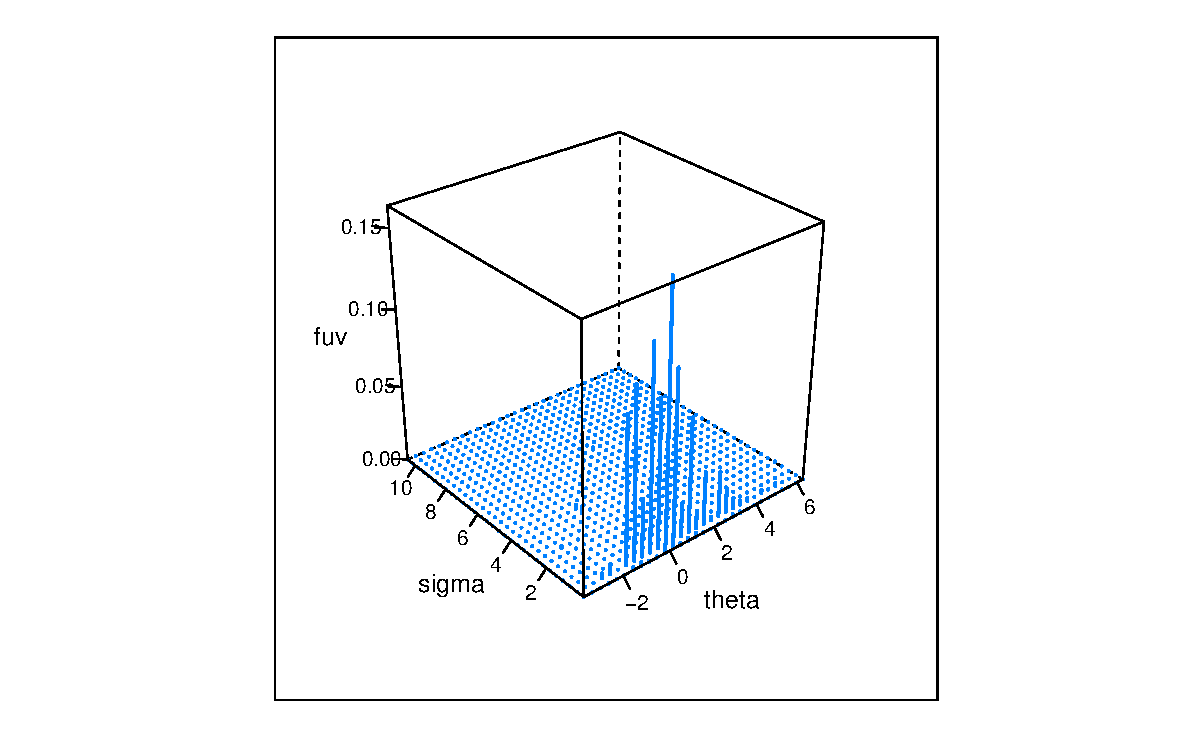
\includegraphics[width=\textwidth]{../../Figures/2013-2022/GMM_m/GLVmix.pdf}
    \end{minipage}\hfill
    \begin{minipage}{0.5\textwidth}
        \centering
        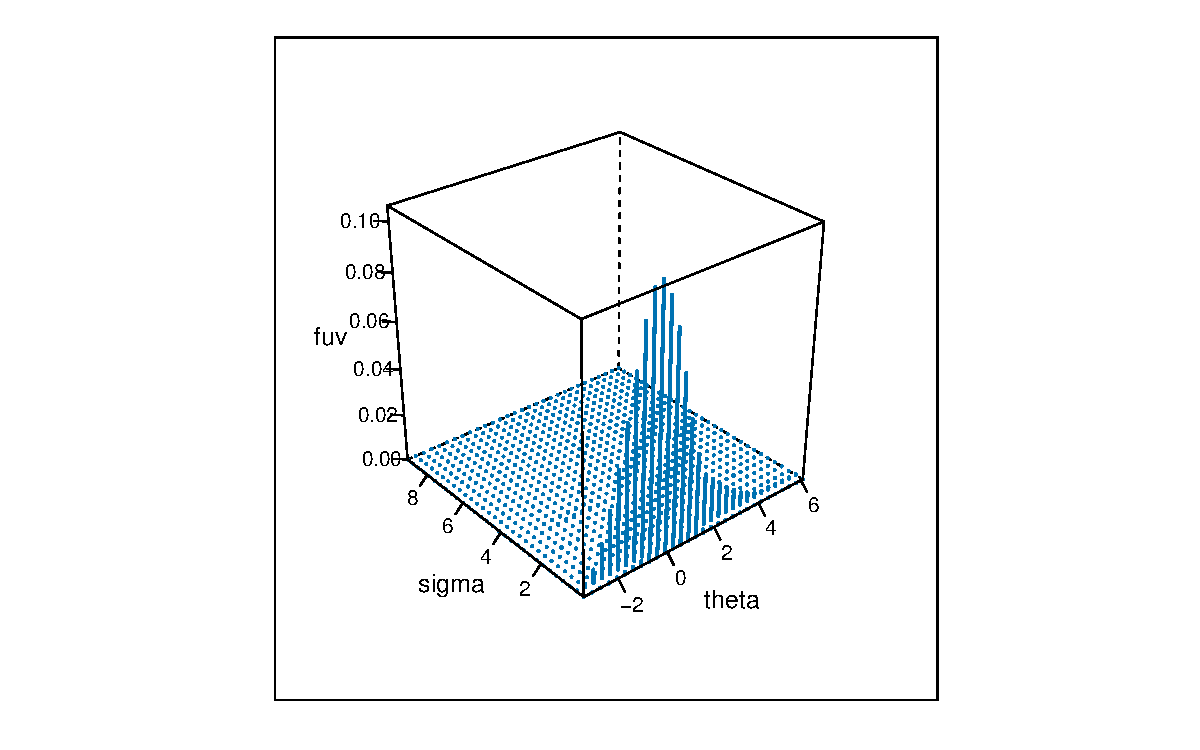
\includegraphics[width=\textwidth]{../../Figures/2013-2022/GMM_m/GLVmix_s.pdf}
    \end{minipage}
\end{figure}

With an estimated prior, the tail probability function as well as the
constraints are well-defined. Though, given the discrete nature of selection,
it is similar to discrete optimization as in knapsack problem. I follow the
approach described in \cite{basu2018weighted} and thus consider only
sequentially selecting the units until one constraint is violated.

In Figure \ref{fig:tp_0.2_0.2_2d}, I present the results of selecting the top
20\% hospitals with or without the FDR constraint at 20\%. The selection rule
is the posterior tail probability which is explained in the sections above,
that is, the solution to the problem defined in \ref{eq:decisionrule}. The
prior $G$ is taken to be the smoothed Kiefer-Wolfowitz estimate.

The left-hand side corresponds to the selection outcome without imposing the
FDR constraints while the right-hand side controls the expected FDR at 20\%. In
the first case, there are around 10 times more private hospitals in the top
20\% while the total number of hospitals is less than twice of the public.

The FDR seems to have only impacted the private hospitals, leaving 18 out of
the selection set. A stringent FDR constraint would lead to a smaller set as
shown in \ref{fig:tp_0.2_0.1_2d}.

\begin{figure}[h!]
    \centering
    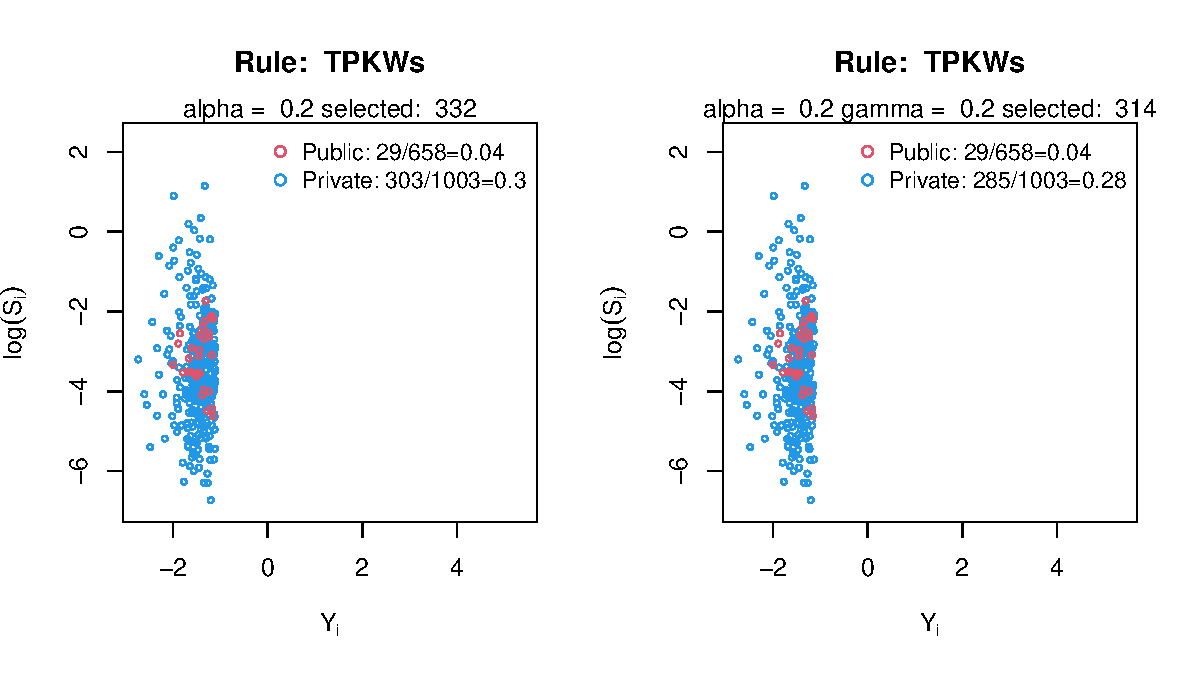
\includegraphics[width=0.8\textwidth]{../../Figures/2013-2022/GMM_m/GLVmix/Left_0.2_0.2_TPKWs.pdf}
    \caption{Tail probability rule, capacity 20\%, FDR 20\%, unknown variance}
    \label{fig:tp_0.2_0.2_2d}
\end{figure}

\begin{figure}[h!]
    \centering
    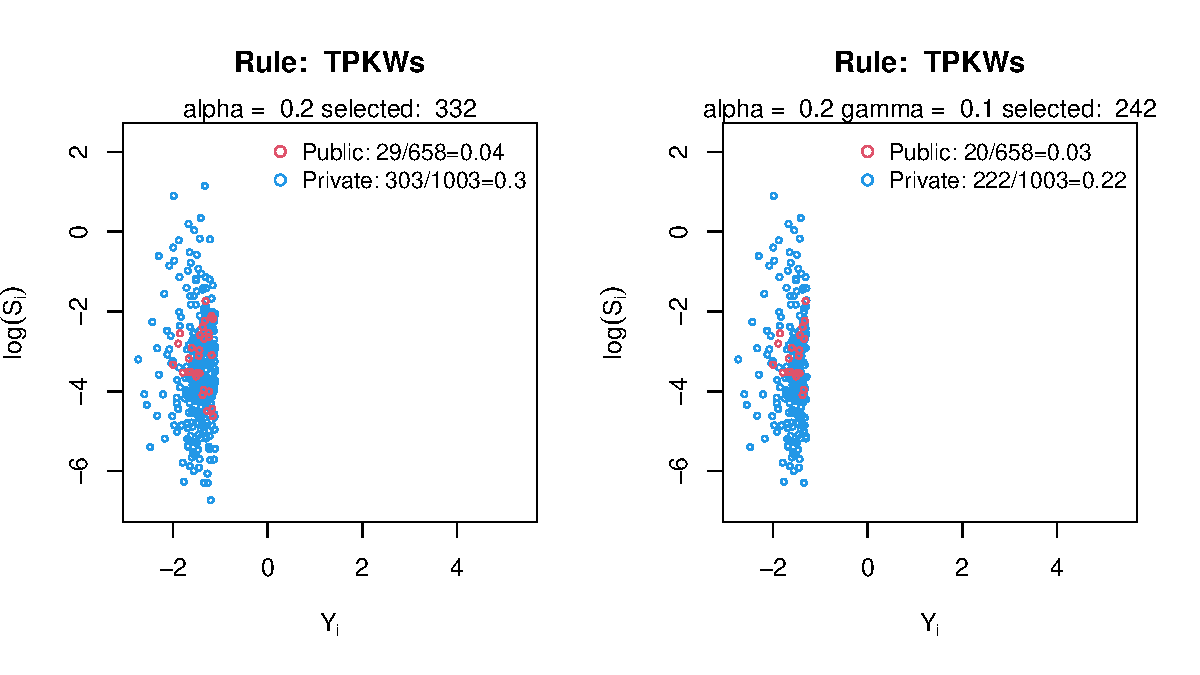
\includegraphics[width=0.8\textwidth]{../../Figures/2013-2022/GMM_m/GLVmix/Left_0.2_0.1_TPKWs.pdf}
    \caption{Tail probability rule, capacity 20\%, FDR 10\%, unknown variance}
    \label{fig:tp_0.2_0.1_2d}
\end{figure}
As of other selection rules using different ranking statistics (posterior mean, MLE face value, James-Stein linear shrinkage), see appendix \ref{section:unknown} for an overview.
\paragraph{Known variance, and TP rules} In \citet{gu2023invidious}, the authors
apply the newly proposed selection method to the the selection of kidney
dialysis centers studied by \citep{lin2006loss,lin2009ranking}. However, the
focus is on the quality of service, specifically on the mortality rate.
Secondly, they assume the predictions of expected mortality is sufficiently
accurate such that the variance is known and independent of $\theta\sim G$.

\begin{figure}[h!]
    \centering
    \begin{minipage}{0.5\textwidth}
        \centering
        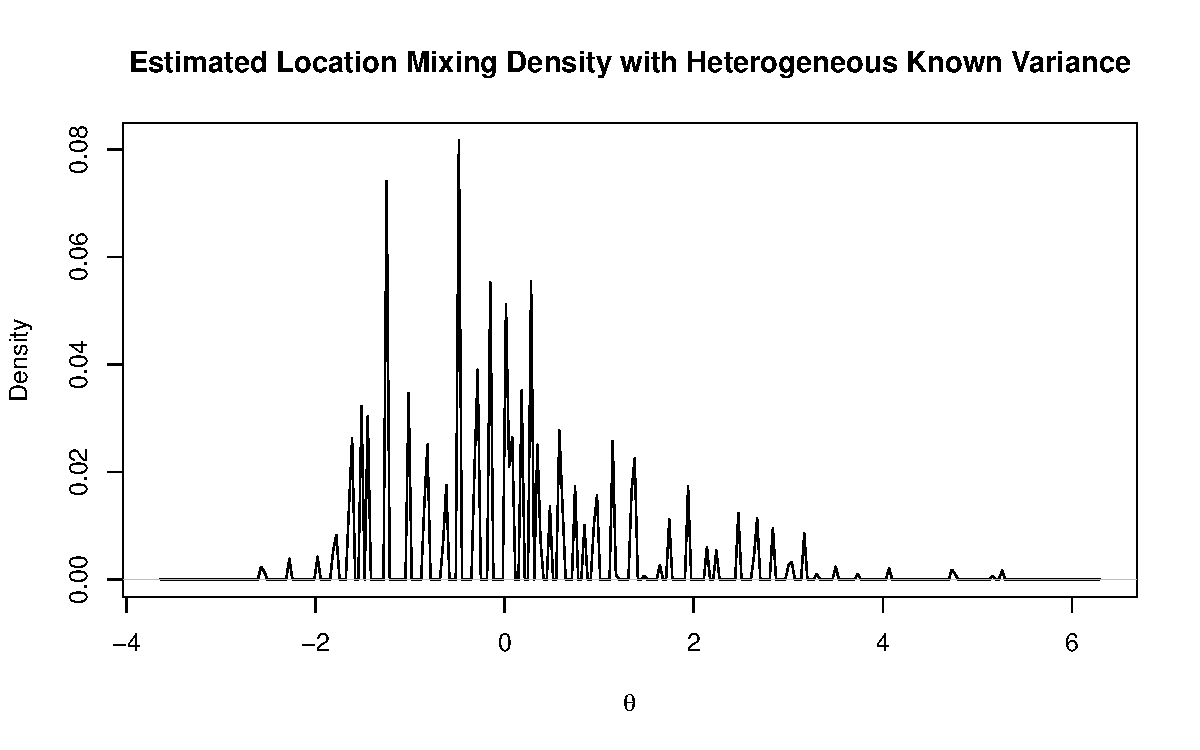
\includegraphics[width=\textwidth]{../../Figures/2013-2022/GMM_m/GLmix.pdf}
    \end{minipage}\hfill
    \begin{minipage}{0.5\textwidth}
        \centering
        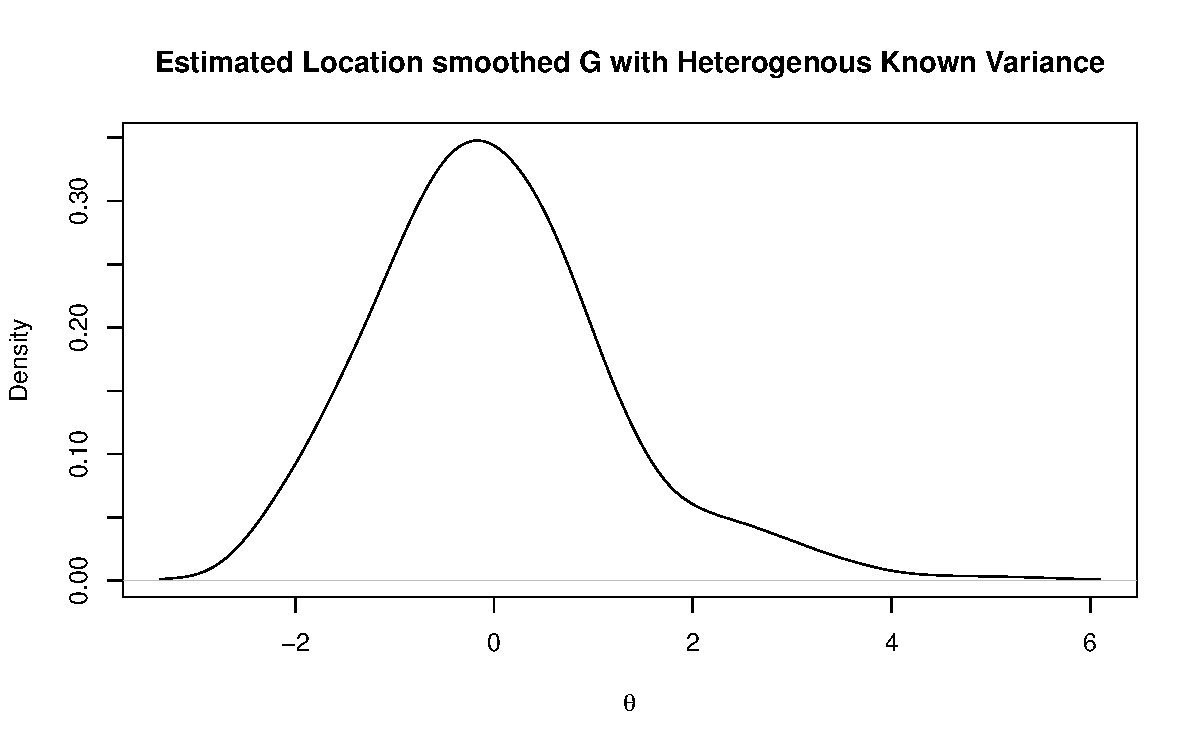
\includegraphics[width=\textwidth]{../../Figures/2013-2022/GMM_m/GLmix_s.pdf}
    \end{minipage}
\end{figure}

Though not desirable in the present setting, it would be interesting to see
what the results would be if I take the $S_i$ as the $\sigma_i^2$. For the
moment, whether this assumption would lead to a more stringent selection
outcome is unclear. Figure \ref{fig:tp_0.2_0.2_1d} presents the outcome under
the posterior tail probability rule with smoothed estimated prior. It seems
that the with only the capacity constraint, the outcome does not differ much.
However, when FDR constraint is combined, the known variance assumption becomes
too lenient to incorporate the newly imposed constraint. At the level
$\alpha=0.2$ and $\gamma=0.2$, the FDR constraint is not binding. While a more
stringent FDR constraint does bind as shwon in Figure \ref{fig:tp_0.2_0.1_1d}.

\begin{figure}[h!]
    \centering
    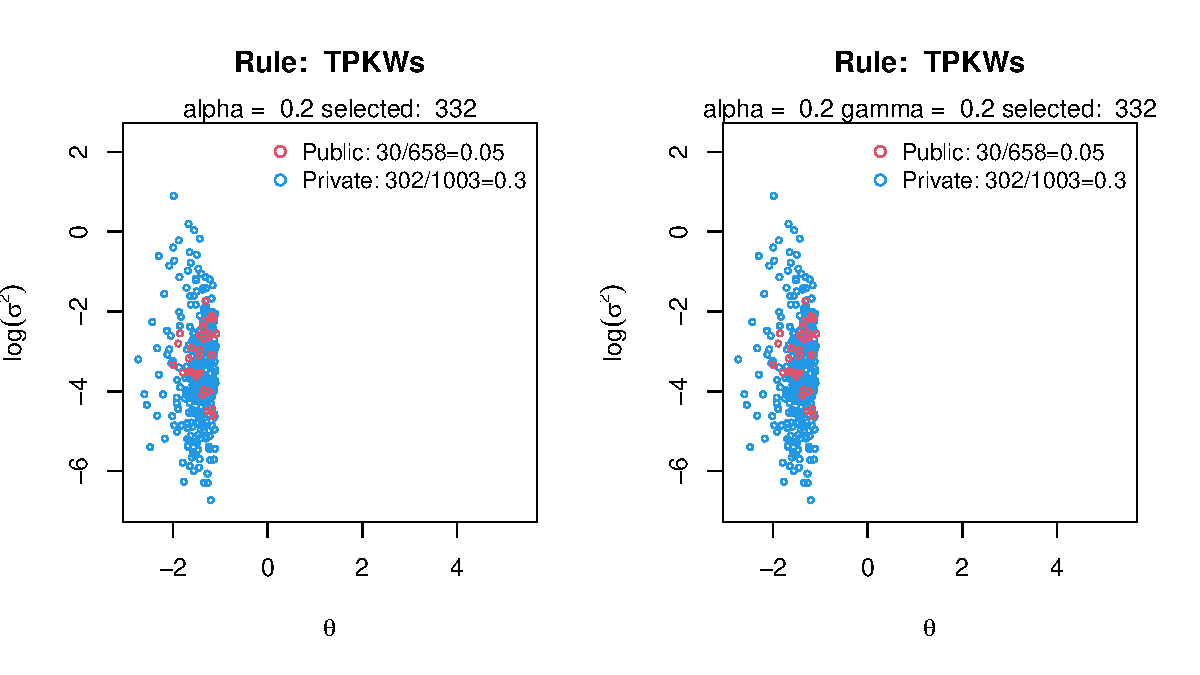
\includegraphics[width=0.8\textwidth]{../../Figures/2013-2022/GMM_m/GLmix/Left_0.2_0.2_TPKWs.pdf}
    \caption{Tail probability rule, capacity 20\%, FDR 20\%, known variance}
    \label{fig:tp_0.2_0.2_1d}
\end{figure}

\begin{figure}[h!]
    \centering
    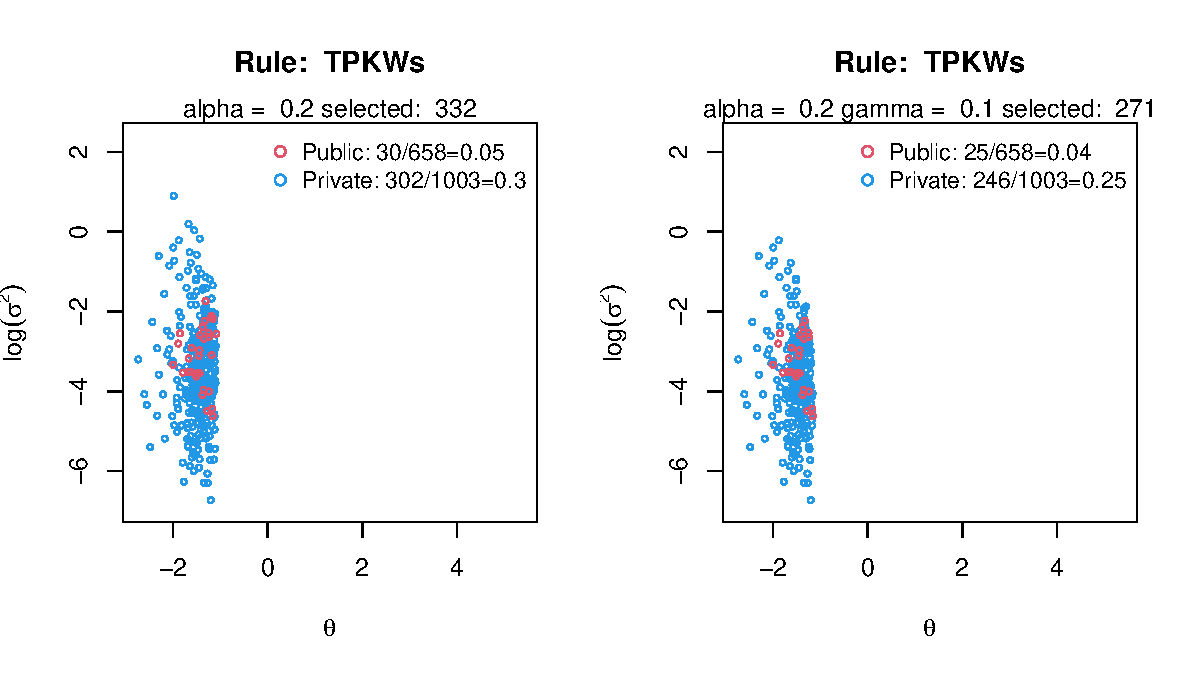
\includegraphics[width=0.8\textwidth]{../../Figures/2013-2022/GMM_m/GLmix/Left_0.2_0.1_TPKWs.pdf}
    \caption{Tail probability rule, capacity 20\%, FDR 10\%, known variance}
    \label{fig:tp_0.2_0.1_1d}
\end{figure}

Appendix \ref{section:known} presents the results of other selection rule. In
this case, a contour line can be drawn to highlight the differences between
ranking statistics.

\section{Conclusion}

Exploiting the rich dataset covering all hospitals in France, I have attempted
to estimate the fixed effect of individual hospitals, which has the
interpretation of \textit{inefficiency index}. Based on an initial estimate, my
goal is to select the top performing hospitals and classify them by legal
status, thereby having a more granular view of the efficiency comparison
between the public and private hospitals. I deliberately omit the teaching
hospitals (~200) from the dataset because they are innately different in terms
of its objectives. To tackle the endogeneity issue, I used lagged difference of
the regressors as instruments for the current level, a simplified version of
the system GMM method. The selection problem of interests falls naturally under
the compound decision framework. Empirical Bayes ideology along with the
developments in nonparametric maximum likelihood estimation has made the
implementation more efficient. In addition to the artificial capacity
constraint where only the top $\alpha\%$ units are of interests, it is an
interesting and useful practice to incorporate the another constraint called
False Discovery Rate constraint such that the expected number of false
posititve is controlled at a certain level. From the application to the French
Hospitals, it is clear that the FDR constraints shrinks the selection set by
some amount. It is also intuitive that the the larger the capacity (larger the
$\alpha$), the less binding the FDR constraint is. The idea is that when the
decision maker can select more units, the probability of making mistakes
decreases. Another observation comes from the assumption we make in the NPMLE
of $G$. In \citet{gu2023invidious}, the authors have pointed out that the known
variance assumption in $Y_i|\theta_i,\sigma_i$ may be plausible in some
applications, it is more common to be faced with only an estimate the variance.
The two assumptions give rise to a different level of \textit{stringency} in
response to the constraints, especially when the decision maker wants to
control for the expected false discovery rate. Assuming an unknown variance
treat the observation as noisier, thus the probability of making mistakes is
higher. The same level of FDR constraint of $20\%$ only binds in the unknown
variance scenario. With respect the private public comparison, among the top
20\% performers, there are around 10 times more private than public, while the
ratio of total number is 5 to 3. A preliminary conclusion is in terms labor
employment efficiency, there are more efficient private hospitals among the top
performers. It may be of interests to the healthcare authority to perform such
selections and take corresponding actions with respect to the selection
outcome. From my point of view, a related report based on the ranking and
selection results will create an incentive for the healthcare providers to
ensure the completeness of data input. sHowever, one cautionary tale is the
interpretation of the fixed effect estimate. Since the fixed effect captures
all time invariant component of the unit, whether it is only the unobserved
heterogeneity of individual hospitals or an actual measure of inefficiency is
of question. The issue is discussed in \citet{greene2005fixed}. Lastly, despite
the fact that it is of human nature to construct ranking and make selections,
every step of the procedure requires attention to the specification,
identification and justifiable assumptions. Incorporating constraints such as
FDR in defining the problem may be helpful, but the decision is still subject
to great uncertainty and should be made with caution and justification.

\pagebreak
\newpage
\bibliography{ref.bib}

\appendix
\section{Appendix}
\subsection{Data}

The panel is first filtered by the following criteria
\begin{enumerate}
    \item the number of nurses is positive,
    \item at least one of STAC inpatient, STAC outpatient, Sessions is positive,
    \item the number of observations is larger than 6
\end{enumerate}
Second, I add one to every variable to avoid null value when taking log.

\subsection{NPMLE $G$}
\citet{koenker2014convex} defined the primal problem as
\begin{equation*}
    \min_{f=dG}\set{-\sum_i \log g(y_i)\bigg |g(y_i) = T(f),\ K(f)=1,\ \forall i }
\end{equation*}
where $ T(f)=\int p(y_i |\theta)fd\theta $ and  $K(f)= \int f d\theta$.\\
By discretizing the support,
\begin{equation*}
    \min_{f=dG}\left\{-\sum_i \log g(y_i)\bigg |g=Af,\ {1^T}f=1\right\}
\end{equation*}
where $A_{ij}= p(y_i|\theta_j) $ and $ f = (f(\theta_1),f(\theta_2),\ldots,f(\theta_m))$.\\
It is straightforward to derive the dual problem
\begin{equation*}
    \max_{\lambda,\mu} \left\{ \sum_i \log \lambda_1(i) \bigg| A^T\lambda_1 < \lambda_2 1,\ (\lambda_1>0) \right\}
\end{equation*}

\subsection{Assumption on $\hat{\theta}_i|\theta_i,\sigma_i$}
If our specification and assumptions on exogeneity are correct, the consistency
of $\hat{\beta}$ is guaranteed by $N$'s asymptotic. However, our estimate of
the fixed effect is
\begin{align*}
    \hat{\theta}_i & =\frac{1}{T}\sum(\theta_i+\varepsilon_{it}+x_{it}(\beta-\hat{\beta}))              \\
                   & \overset{N\to \infty}{\longrightarrow} \theta_i+\frac{1}{T}\sum_t \varepsilon_{it} \\
\end{align*}
When $T$ is relatively small (or even fixed), I am not in a good position to use central limit theorem to claim that $\hat{\theta}_i \overset{d}{\to} \caln(\theta_i,\frac{\sigma_i^2}{T})$. A bold assumption that $\varepsilon_{it} \sim \caln(0,\sigma_i^2)$ will save me from the $T$ issue, which I will impose for the rest of the section (and abstract from whether that  for each $i$ is a testable/reasonable/feasible assumption).

\subsection{Comparison of selection rules}

\newpage
\subsubsection{Unknown variance}
\label{section:unknown}

\begin{figure}[h!]
    \centering
    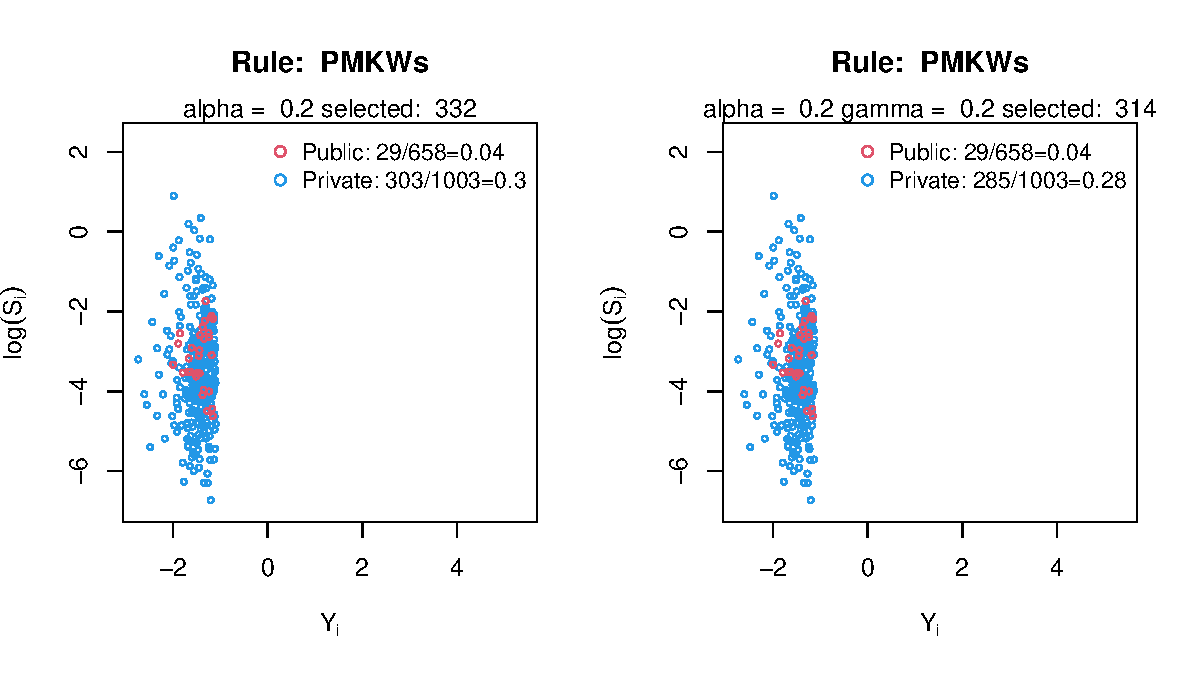
\includegraphics[width=0.8\textwidth]{../../Figures/2013-2022/GMM_m/GLVmix/Left_0.2_0.2_PMKWs.pdf}
    \caption{Posterior mean, capacity 20\%, FDR 20\%, unknown variance}
\end{figure}

\begin{figure}[h!]
    \centering
    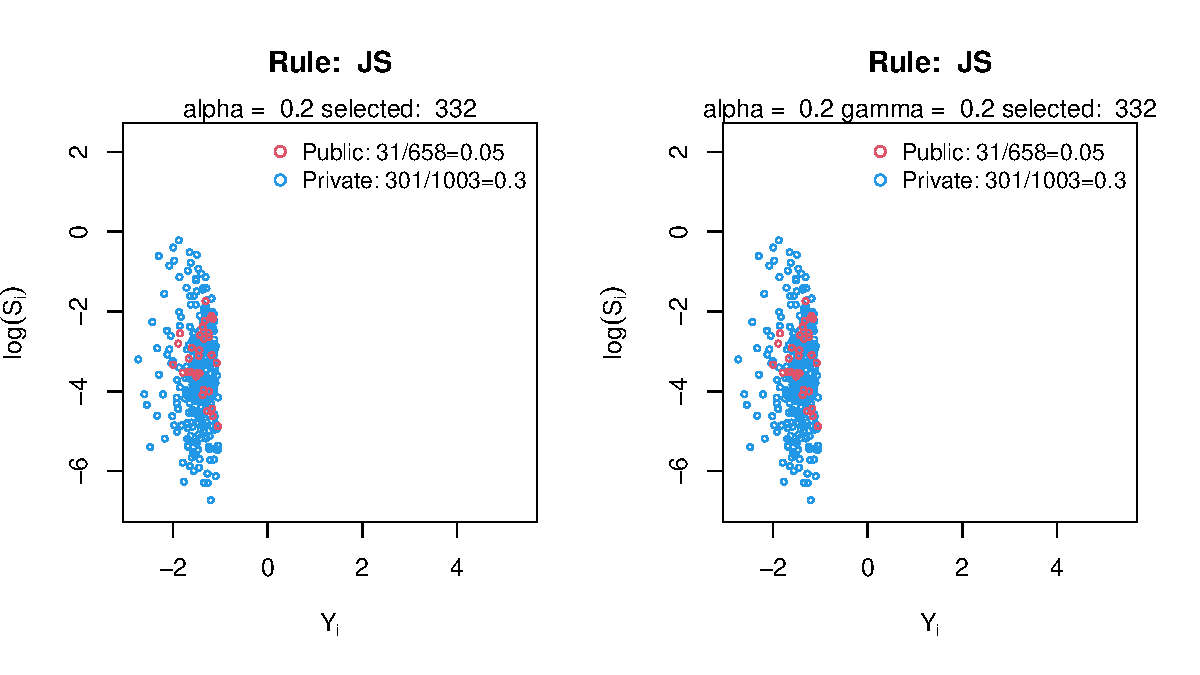
\includegraphics[width=0.8\textwidth]{../../Figures/2013-2022/GMM_m/GLVmix/Left_0.2_0.2_JS.pdf}
    \caption{James-Stein Linear Shrinkage, capacity 20\%, FDR 20\%, unknown variance}
\end{figure}

\begin{figure}[h!]
    \centering
    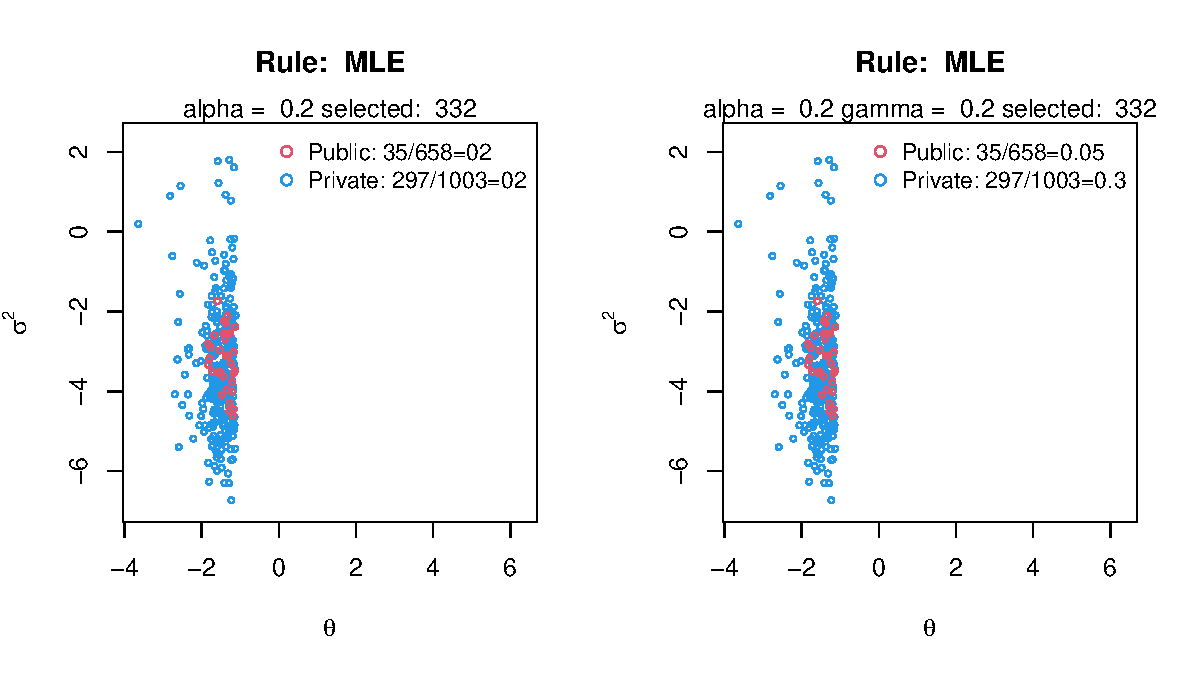
\includegraphics[width=0.8\textwidth]{../../Figures/2013-2022/GMM_m/GLVmix/Left_0.2_0.2_MLE.pdf}
    \caption{MLE, capacity 20\%, FDR 20\%, known variance}
\end{figure}

\newpage
\subsubsection{Known variance}
\label{section:known}
\begin{figure}[h!]
    \centering
    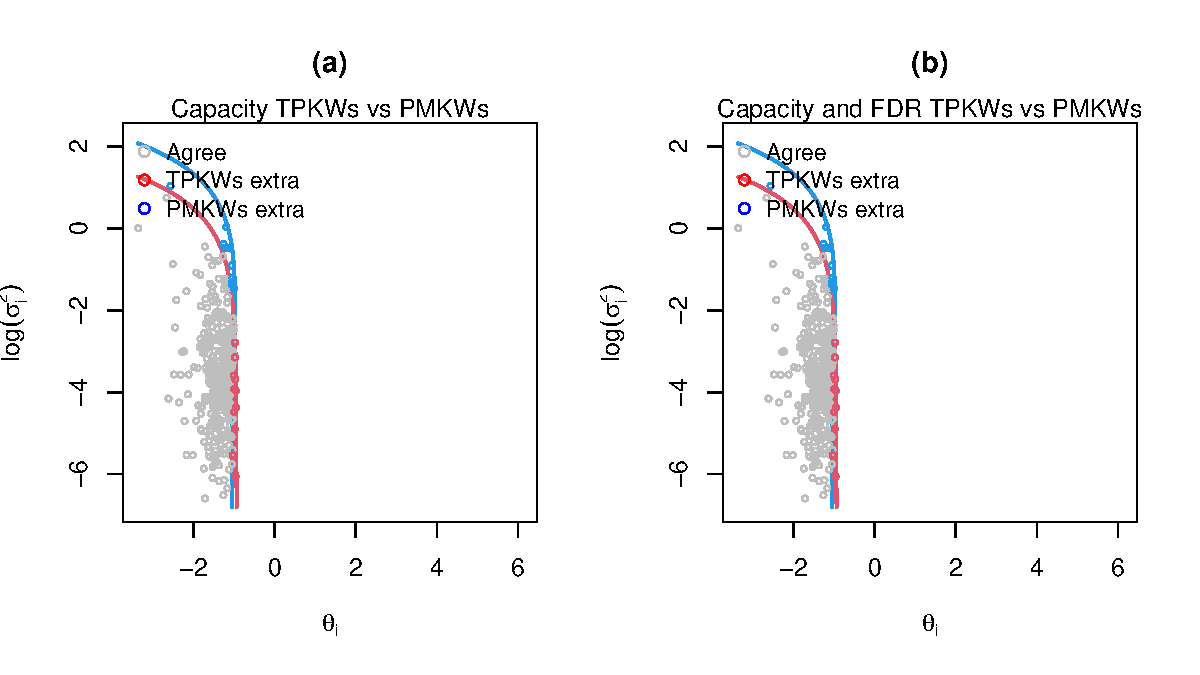
\includegraphics[width=0.8\textwidth]{../../Figures/2013-2022/GMM_m/GLmix/Contour_Left_0.2_0.2_TPKWs_PMKWs.pdf}
    \caption{TP VS PM,  capacity 20\%, FDR 20\%, known variance}
\end{figure}

\begin{figure}[h!]
    \centering
    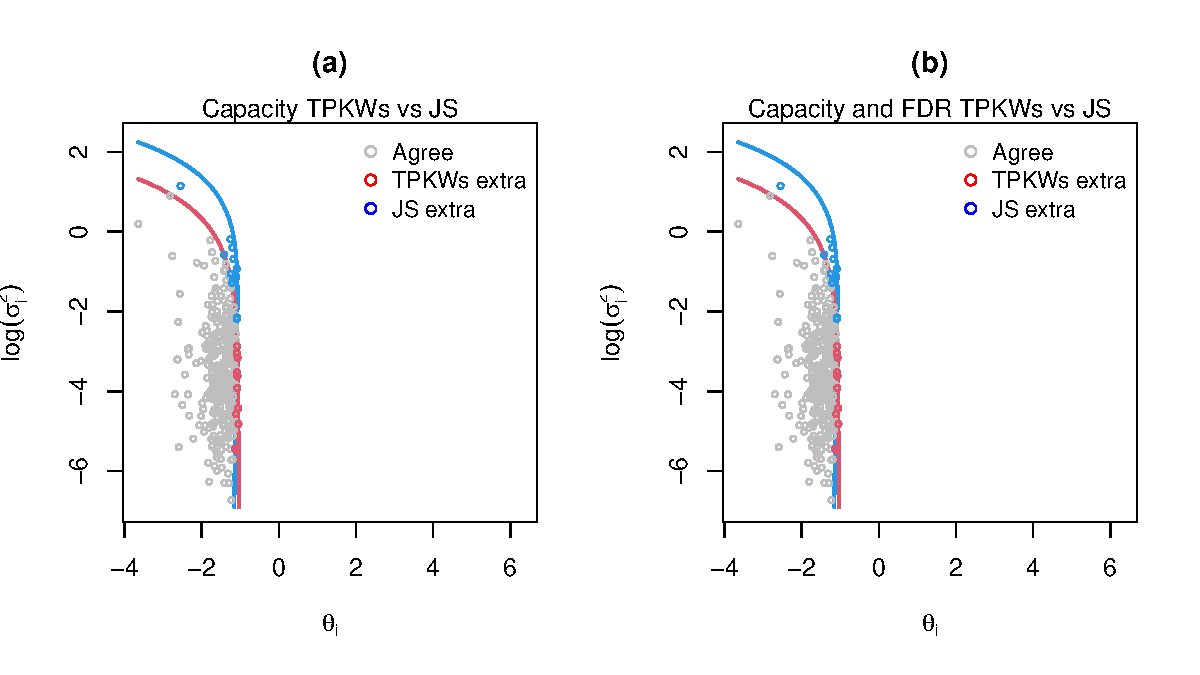
\includegraphics[width=0.8\textwidth]{../../Figures/2013-2022/GMM_m/GLmix/Contour_Left_0.2_0.2_TPKWs_JS.pdf}
    \caption{TP VS JS, capacity 20\%, FDR 20\%, known variance}
\end{figure}

\begin{figure}[h!]
    \centering
    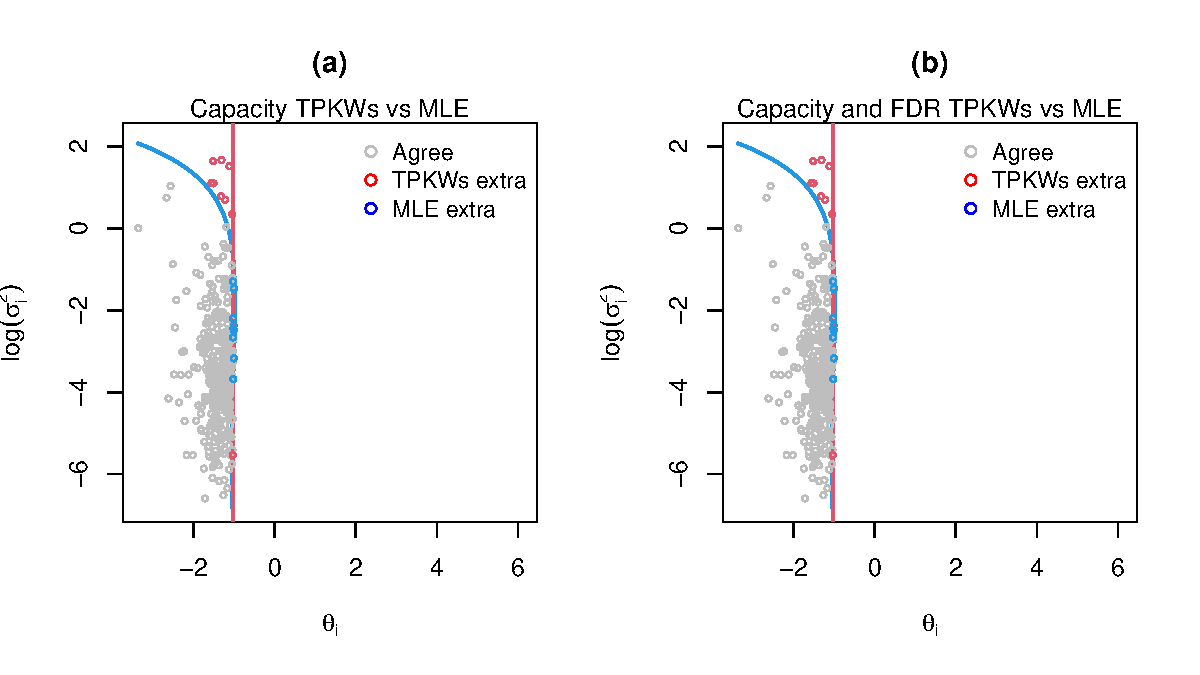
\includegraphics[width=0.8\textwidth]{../../Figures/2013-2022/GMM_m/GLmix/Contour_Left_0.2_0.2_TPKWs_MLE.pdf}
    \caption{TP VS MLE, capacity 20\%, FDR 20\%, unknown variance}
\end{figure}

\end{document}